\subsection{Heurística 1: distancia al alimento más lejano}

Es exactamente la fórmula que sugiere la guía como primera aproximación:
$h(n) = \max_{f \in F} d_M(n, f)$, la distancia Manhattan desde la posición actual hasta el
alimento restante más lejano.

\begin{figure}[H]
\centering
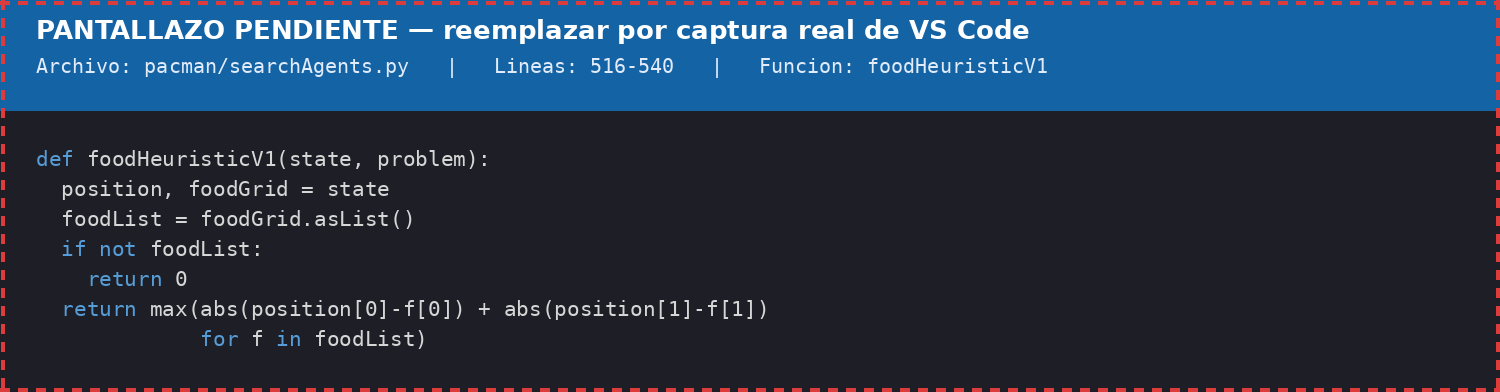
\includegraphics[width=0.85\textwidth]{capturas/actividad11_heuristica1.png}
\caption{\texttt{foodHeuristicV1} en \texttt{pacman/searchAgents.py} (líneas 516-540).}
\label{fig:act11-h1}
\end{figure}

\textbf{Admisibilidad:} el costo real para recoger toda la comida restante es, como mínimo, el
costo de llegar hasta el alimento más lejano --en algún momento del recorrido Pac-Man tiene que
llegar hasta él--, y la distancia Manhattan nunca sobreestima una distancia real en una cuadrícula
con paredes. Por lo tanto $h(n) \le h^*(n)$ siempre.

\textbf{Consistencia:} para cualquier sucesor $n'$ de $n$ (un paso ortogonal, costo 1), si el
alimento más lejano de $n$ sigue presente en $n'$ (no fue el que se acaba de comer), la desigualdad
triangular de Manhattan da $d_M(n,f^*) \le d_M(n,n') + d_M(n',f^*) = 1 + d_M(n',f^*) \le 1 + h(n')$.
Si el alimento más lejano de $n$ era justo el que estaba en $n'$ (se acaba de comer),
$d_M(n,n') = 1 \le 1 + h(n')$ porque $h(n') \ge 0$ siempre. En ambos casos $h(n) \le 1 + h(n')$.

\subsection{Heurística 2: diámetro Manhattan de posición + comida restante}

Generaliza la Heurística 1: en vez de mirar solo la distancia de Pac-Man al alimento más lejano,
considera el \textbf{diámetro} (la mayor distancia Manhattan entre cualquier par) del conjunto
formado por la posición actual \emph{más} todos los alimentos restantes:

$$h(n) = \max\Big(\max_{f \in F} d_M(n,f), \ \max_{f_i, f_j \in F} d_M(f_i, f_j)\Big)$$

Es más informativa que la Heurística 1 porque también considera que, para visitar dos alimentos
lejanos entre sí, Pac-Man tiene que recorrer al menos la distancia real entre ellos en algún
momento del camino --no solo la distancia desde su posición actual hasta el más lejano de los dos--.

\begin{figure}[H]
\centering
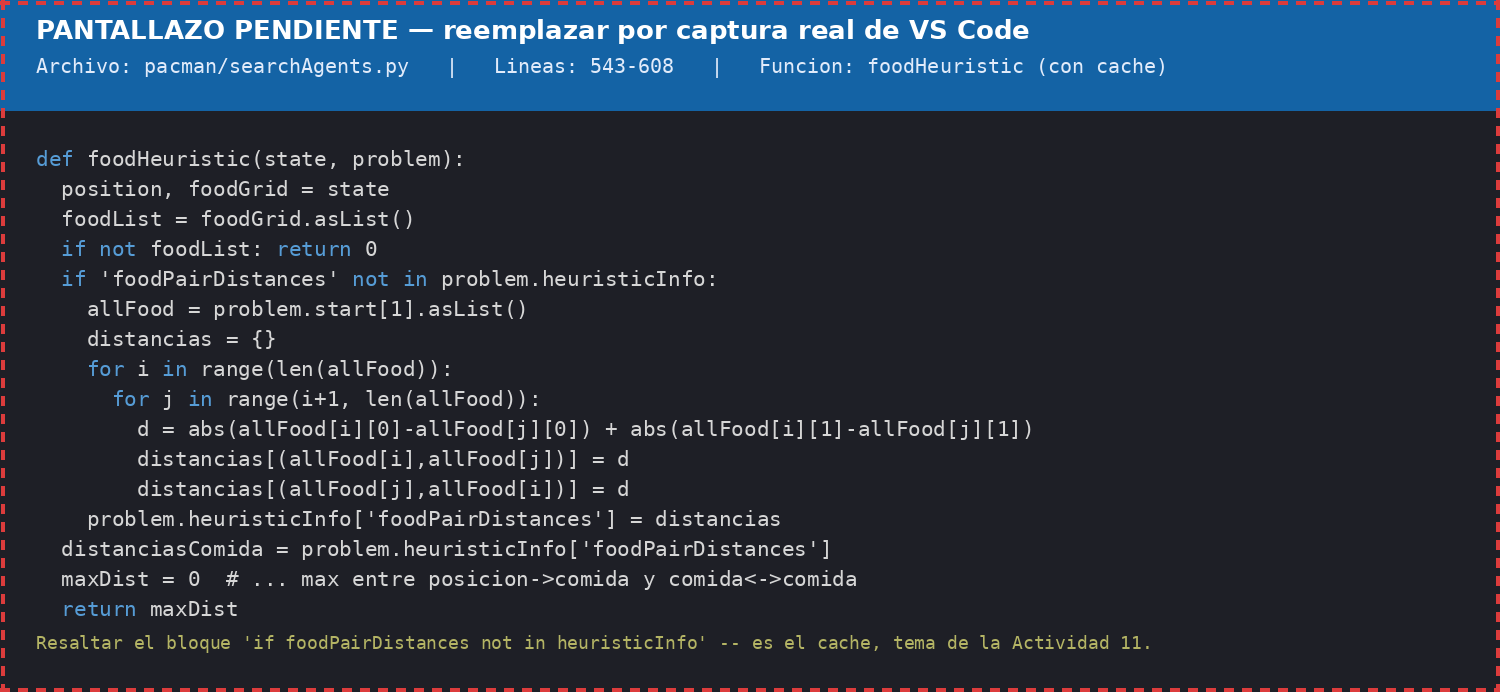
\includegraphics[width=0.9\textwidth]{capturas/actividad11_heuristica2.png}
\caption{\texttt{foodHeuristic} (Heurística 2, con caché en \texttt{problem.heuristicInfo}) en
\texttt{pacman/searchAgents.py} (líneas 543-608). El bloque
\texttt{if 'foodPairDistances' not in problem.heuristicInfo} es el caché discutido más abajo.}
\label{fig:act11-h2}
\end{figure}

\textbf{Admisibilidad:} el recorrido que visita, en cualquier orden, la posición $n$ y todos los
alimentos de $F$ tiene una longitud real que es, como mínimo, la distancia real entre el par de
puntos (de $\{n\} \cup F$) más separado entre sí --en algún momento del recorrido Pac-Man pasa por
ambos puntos de ese par--. Como la distancia Manhattan nunca sobreestima la distancia real, el
diámetro en Manhattan de $\{n\} \cup F$ es una cota inferior válida: $h(n) \le h^*(n)$.

\textbf{Consistencia:} el mismo argumento de desigualdad triangular de la Heurística 1 se aplica
aquí a cualquier par de puntos de $\{n, n'\} \cup F$. El caso más delicado es cuando se acaba de
comer el alimento en $n'$ (es decir, $F' = F \setminus \{n'\}$ tras el paso): como
$\{n\} \cup F = \{n, n'\} \cup F'$, para cualquier par que incluya a $n$ y a algún
$q \in \{n'\} \cup F'$ se cumple $d_M(n,q) \le d_M(n,n') + d_M(n',q) = 1 + d_M(n',q) \le 1 + h(n')$
(porque $q \in \{n'\} \cup F'$ acota por el máximo); si el par no incluye a $n$, ya está dentro de
$\{n'\} \cup F'$ y su distancia es, por definición, $\le h(n')$. Por lo tanto $h(n) \le 1 + h(n')$
en todos los casos, y $h(\text{meta}) = 0$ porque con $F=\emptyset$ el conjunto $\{n\}$ es un único
punto (diámetro 0).

\subsection{Optimización con \texttt{problem.heuristicInfo}: qué se cachea y por qué}

El cálculo que se repite en \emph{cada} llamada a la heurística (una por cada nodo expandido,
potencialmente miles de veces) es la distancia Manhattan entre cada \emph{par} de alimentos. Pero
las posiciones de los alimentos nunca cambian durante la búsqueda --solo si siguen presentes o
no--, así que esas distancias se calculan una sola vez (para todos los pares del layout inicial,
usando \texttt{problem.start[1]}, el \texttt{foodGrid} original) y se guardan en
\texttt{problem.heuristicInfo['foodPairDistances']}; las llamadas siguientes reutilizan ese
diccionario en vez de recalcular la fórmula de distancia para el mismo par de alimentos.

\subsection{Procedimiento y resultados}

Se ejecutó A* con las tres heurísticas ($h(n)=0$, Heurística 1, Heurística 2) sobre
\texttt{tinySearch} y \texttt{testClassic} (ver \texttt{experimentos/actividad11\_food\_heuristic.py}).

\begin{table}[H]
\centering
\caption{Comparación de heurísticas de comida sobre \texttt{testClassic} (8 alimentos)}
\label{tab:act11-comparacion}
\begin{tabular}{lrrrr}
\toprule
\textbf{Heurística} & \textbf{Costo} & \textbf{Longitud} & \textbf{Expandidos} & \textbf{Tiempo (s)} \\
\midrule
$h(n)=0$      & 16 & 16 & 2598 & 0.070222 \\
Heurística 1  & 16 & 16 &  702 & 0.024714 \\
Heurística 2  & 16 & 16 &  383 & 0.014872 \\
\bottomrule
\end{tabular}
\end{table}

En \texttt{tinySearch} (1 alimento) las tres coinciden en costo (8) y las dos heurísticas empatan
en 8 nodos expandidos frente a los 16 de $h(n)=0$ --con un solo alimento no hay ninguna pareja de
alimentos que comparar, así que la Heurística 2 se reduce exactamente a la Heurística 1--. La
diferencia real aparece en \texttt{testClassic}: la Heurística 1 ya reduce drásticamente la
exploración frente a $h(n)=0$ (2598 $\rightarrow$ 702, factor $R \approx 3.70$), y la Heurística 2
la reduce aún más (2598 $\rightarrow$ 383, factor $R \approx 6.78$; 319 nodos menos que la
Heurística 1), confirmando que considerar también la distancia entre pares de alimentos --no solo
la distancia desde Pac-Man-- aporta información adicional real, no solo teórica.

\subsection{El reto del caché: qué encontramos (y por qué es un resultado honesto, no un error)}

Comparamos el tiempo de A*+Heurística~2 con caché (\texttt{foodHeuristic}) contra una versión
idéntica pero sin caché (\texttt{foodHeuristicV2SinCache}, que recalcula las distancias entre pares
de alimentos restantes en cada llamada), promediando 5 corridas por versión en dos layouts:

\begin{table}[H]
\centering
\caption{Heurística 2 con caché vs. sin caché (tiempo promedio de 5 corridas)}
\label{tab:act11-cache}
\begin{tabular}{lrrr}
\toprule
\textbf{Layout (alimentos)} & \textbf{Expandidos} & \textbf{Tiempo con caché (s)} & \textbf{Tiempo sin caché (s)} \\
\midrule
testClassic (8)    & 383  & 0.015458 & 0.014835 \\
capsuleClassic (23) & 2185 & 0.207050 & 0.193121 \\
\bottomrule
\end{tabular}
\end{table}

El resultado es contraintuitivo pero reproducible: la versión \emph{sin} caché fue, en ambos casos,
ligeramente \emph{más rápida} (entre 4\% y 7\%), no más lenta. La explicación no es que el caché
esté mal implementado --los nodos expandidos son idénticos en ambas versiones, porque es
exactamente la misma heurística--, sino que el cálculo que se está cacheando es demasiado barato
para que valga la pena: son sumas y restas de enteros (\texttt{abs(f1[0]-f2[0]) + abs(f1[1]-f2[1])}),
mientras que consultar el diccionario \texttt{problem.heuristicInfo['foodPairDistances']} implica
construir una tupla \texttt{(f1, f2)} como llave y calcular su hash en cada consulta. En este
problema, con a lo sumo un par de decenas de alimentos, el costo de esa búsqueda en el diccionario
termina siendo comparable --o incluso mayor-- al costo de simplemente recalcular la resta. El
caché con \texttt{problem.heuristicInfo} sigue siendo la herramienta correcta que sugiere la guía,
pero su beneficio depende de que el cálculo evitado sea realmente costoso (por ejemplo, una
distancia real de laberinto calculada con BFS en vez de una resta Manhattan); aquí, honestamente,
no lo es. Dejamos ambas versiones en el código (\texttt{foodHeuristic} con caché se usa en
\texttt{AStarFoodSearchAgent}, y \texttt{foodHeuristicV2SinCache} existe solo para esta comparación)
precisamente para poder mostrar esta medición en vivo si se pide en la sustentación.
